\subsection{Excercise DockerEnvironmentSetup}
This exercise sets up the Docker environment.
The goal is to install Docker and run the Hello-World container.

First, Docker is installed on the author's machine.
A quick verification is done to ensure that the installation was successful.
After that, the Hello-World container is run twice explaining the differences between the first and second execution.

\subsubsection*{Installing Docker}
The installation is carried out on the author's machine running Windows 11 with WSL2.
The installation is done by following the official Docker documentation \cite{DO-INST} and the provided guide on the task sheet \cite{CM-G-BSD}.

After successfully installing Docker, the installation is verified by running \texttt{docker \-\-version} and \texttt{docker-compose \-\-version} in the terminal.
The output of the commands is shown in \autoref*{fig:docker_installation_verification}.

\begin{figure}
    \centering
    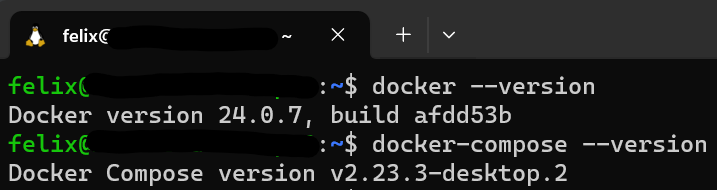
\includegraphics[width=0.8\textwidth]{figures/microservices/dmCar/ms_dmCar_dockerInstallation.png}
    \caption{Docker Installation Verification}
    \label{fig:docker_installation_verification}
\end{figure}
\subsubsection*{Running Hello-World Container}
The next step is to run the Hello-World container.
This is done by running the \texttt{docker run hello-world} command in the terminal.
The command is executed twice showing the differences between both executions.

Execution one is shown in \autoref*{fig:docker_hello_world_first_execution}.
The output shows that the image needed for the container is not available locally at first.
Therefore, the image is pulled automatically from the Docker Hub.
Afterwards, the container is started and the output is shown.

The second execution is shown in \autoref*{fig:docker_hello_world_second_execution}.
Here, the image is already available locally and therefore, no new image needs to be pulled from the Docker Hub.
The container is started instantly and the same output is shown.

\begin{figure}
    \centering
    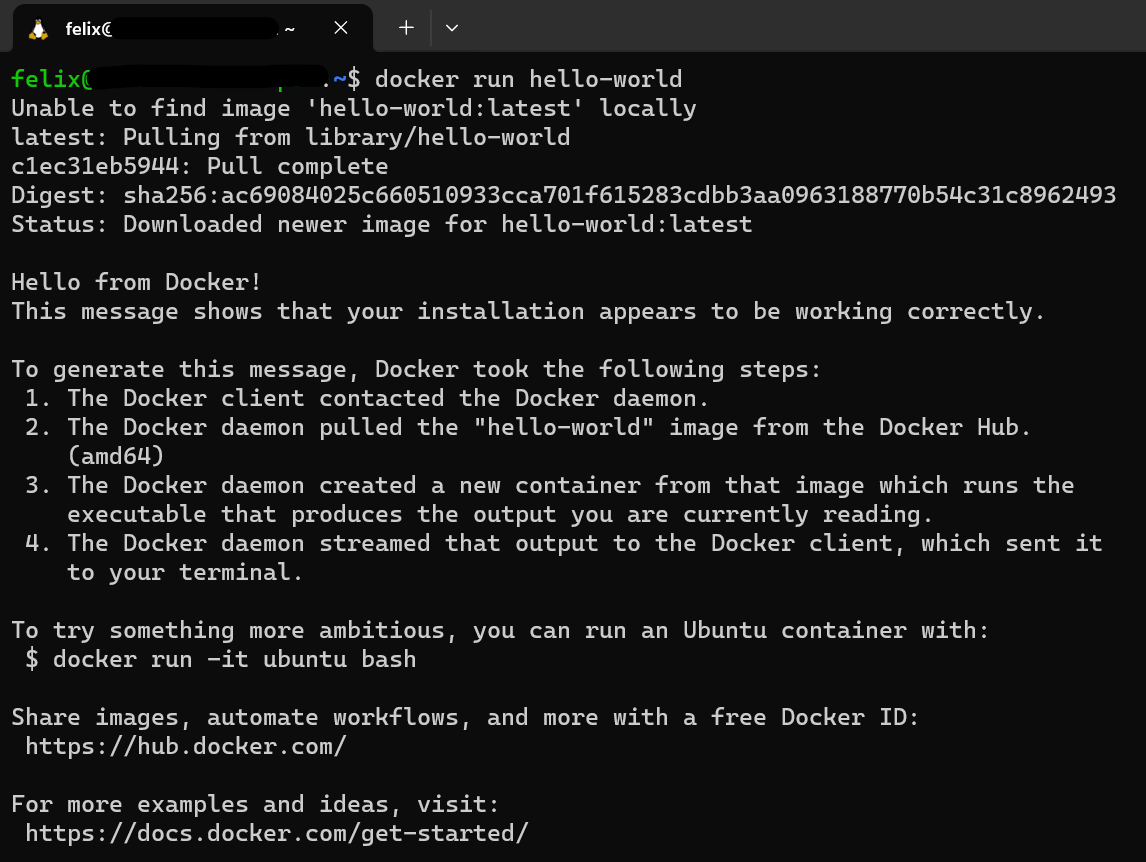
\includegraphics[width=0.6\textwidth]{figures/microservices/dmCar/ms_dmCar_dockerHelloWorldFirstExecution.png}
    \caption{First Execution of Hello-World Container}
    \label{fig:docker_hello_world_first_execution}
\end{figure}

\begin{figure}
    \centering
    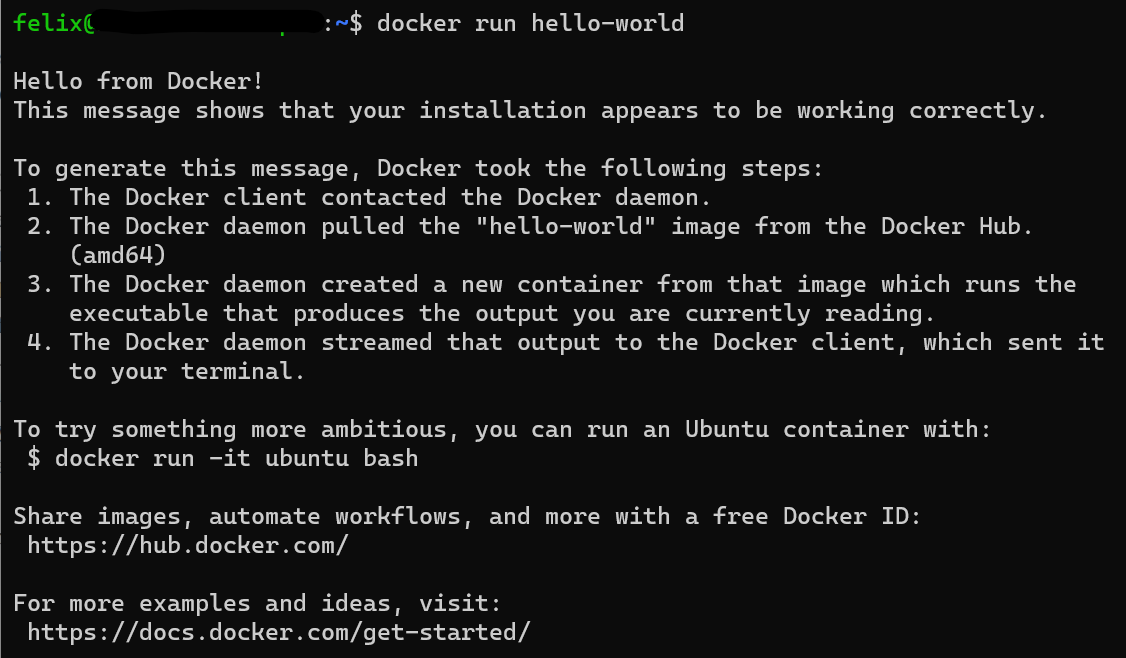
\includegraphics[width=0.6\textwidth]{figures/microservices/dmCar/ms_dmCar_dockerHelloWorldSecondExecution.png}
    \caption{Second Execution of Hello-World Container}
    \label{fig:docker_hello_world_second_execution}
\end{figure}

%==============================================================================

\subsection{Excercise DockerContainerization}
//TODO add introduction
\subsubsection*{Add Dockerfile to DM-Car}

\subsubsection*{Familiarize With Dockerfile Syntax}


\subsubsection*{Build Docker Image}


\subsubsection*{Optimize Image}


\subsubsection*{Build Optimized Image}


\subsubsection*{Define a File .dockerignore}